%!TEX TS-program = xelatex
%!TEX encoding = UTF-8 Unicode

\documentclass[10pt,twocolumn,oneside]{article}
\usepackage[bmargin=12in]{geometry}
\setlength{\columnsep}{16pt}
\setlength{\columnseprule}{0pt} 

\usepackage{fontspec}
\usepackage{color}
\usepackage[x11names]{xcolor}
\usepackage{CJKutf8} 
\usepackage{amsmath, courier, listings, fancyhdr, graphicx}
%\topmargin=0pt
\headsep=5pt
\textheight=740pt
\footskip=0pt
\voffset=-42pt
\textwidth=545pt
\marginparsep=0pt
\marginparwidth=0pt
\marginparpush=0pt
\oddsidemargin=0pt
\evensidemargin=0pt
\hoffset=-42pt

\setmainfont{Consolas}              
\setmonofont{Consolas}              
%\setmainfont{sourcecodepro}
\XeTeXlinebreaklocale "zh"                      
\XeTeXlinebreakskip = 0pt plus 1pt              
\setcounter{secnumdepth}{3}                     



\lstset{                                            
    language=C++,                                   % the language of the code
    basicstyle=\footnotesize,                       % the size of the fonts that are used for the code
    numbers=left,                                   % where to put the line-numbers
    numberstyle=\footnotesize,                      % the size of the fonts that are used for the line-numbers
    stepnumber=1,                                   % the step between two line-numbers. If it's 1, each line  will be numbered
    numbersep=4pt,                                  % how far the line-numbers are from the code
    backgroundcolor=\color{white},                  % choose the background color. You must add \usepackage{color}
    showspaces=false,                               % show spaces adding particular underscores
    showstringspaces=false,                         % underline spaces within strings
    showtabs=false,                                 % show tabs within strings adding particular underscores
    frame=false,                                    % adds a frame around the code
    tabsize=2,                                      % sets default tabsize to 2 spaces
    captionpos=b,                                   % sets the caption-position to bottom
    breaklines=true,                                % sets automatic line breaking
    breakatwhitespace=false,                        % sets if automatic breaks should only happen at whitespace
    escapeinside={\%*}{*)},                         % if you want to add a comment within your code
        morekeywords={*},                               % if you want to add more keywords to the set
        keywordstyle=\bfseries\color{Blue1},
        commentstyle=\itshape\color{Red4},
        stringstyle=\itshape\color{Green4}
    }



    \begin{document}
    \pagestyle{fancy}
    \fancyfoot{}
    %\fancyfoot[R]{\includegraphics[width=20pt]{ironwood.jpg}}
    \fancyhead[L]{National Chiao Tung University Aurora}
    \fancyhead[R]{\thepage}
    \renewcommand{\headrulewidth}{0.4pt}
    \renewcommand{\contentsname}{Codebook} 

    \scriptsize
    \tableofcontents

    \newpage

    \section{Basic}
    \subsection{vimrc}
    \lstinputlisting{./../codebook/basic/vimrc}
    \subsection{stack increase}
    \lstinputlisting{./../codebook/basic/stack.cpp}
    \subsection{Extc++}
    \lstinputlisting{./../codebook/basic/extc++.cpp}
    \newpage


    \section{Number}
    \subsection{Extended GCD}
    \lstinputlisting{./../codebook/math/number/ext_gcd.cpp}
    \subsection{Modular Inverse}
    \lstinputlisting{./../codebook/math/number/mod_inverse.cpp}
    \subsection{Line Modular Equation}
    \lstinputlisting{./../codebook/math/number/line_mod_equation.cpp}
    \subsection{Chinese Remainder Theorem}
    \lstinputlisting{./../codebook/math/number/crt.cpp}
    \subsection{C(N,M)}
    \lstinputlisting{./../codebook/math/number/C_NM.cpp}
    \subsection{Phi}
    \lstinputlisting{./../codebook/math/number/phi.cpp}
    \subsection{Mul Mod}
    \lstinputlisting{./../codebook/math/number/mul_mod.cpp}
    \subsection{Pollard Rho}
    \lstinputlisting{./../codebook/math/number/pollard_rho.cpp}
    \subsection{Miller Rabin}
    \lstinputlisting{./../codebook/math/number/miller_rabin.cpp}
    \subsection{FFT}
    \lstinputlisting{./../codebook/math/number/fft.cpp}
    \subsection{Function}
    \lstinputlisting{./../codebook/math/number/function.cpp}
    \subsection{Equation}
    \lstinputlisting{./../codebook/math/number/equation.cpp}
    \subsection{Permutation}
    \lstinputlisting{./../codebook/math/number/permutation.cpp}
    \subsection{Catalan Number}
    %!TEX TS-program = xelatex
%!TEX encoding = UTF-8 Unicode
$C_{0}=1$ and $C_{n+1}=\sum_{i=0}^{n}C_{i}C_{n-i}=\frac{2(2n+1)}{n+2}C_{n}$ for $n\ge0$\\
$C_{n}=\frac{1}{n+1}\sum_{i=0}^{n}\binom{n}{i}^{2}=\frac{1}{n+1}\binom{2n}{n}=\binom{2n}{n}-\binom{2n}{n+1}$ for $n\ge0$


    \subsection{Long PI}
    \lstinputlisting{./../codebook/math/number/longpi.py}
    \subsection{Simplex}
    \lstinputlisting{./../codebook/math/number/simplex.cpp}
    %\newpage

    \section{Matrix}
    \subsection{Guass Elimination}
    \subsection{Solve Matrix (Ax=B)}
    \subsection{Inverse Matrix}
    \lstinputlisting{./../codebook/math/matrix/matrix.cpp}
    \subsection{Conjugate Gradient}
    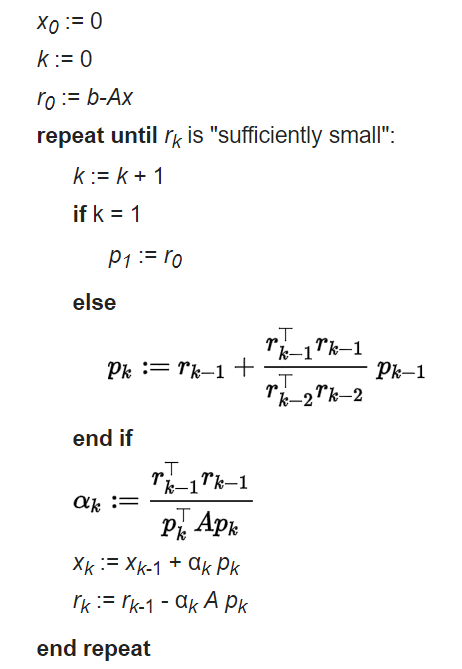
\includegraphics{./../codebook/math/matrix/cg.png}
    %\newpage


    \section{Graph}
    %\subsection{Bridge And Cut}
    %\lstinputlisting{./../codebook/graph/cut_bridge.cpp}
    %\subsection{BCC}
    %\lstinputlisting{./../codebook/graph/bcc.cpp}
    %\subsection{SCC}
    %\lstinputlisting{./../codebook/graph/scc.cpp}
    %\subsection{Two Sat}
    %\lstinputlisting{./../codebook/graph/twosat.cpp}
    \subsection{Maximal Clique}
    \lstinputlisting{./../codebook/graph/bron_kerbosch.cpp}
    %\newpage

    \section{Path}
    \subsection{Dijkstra}
    \subsection{Kth Shortest}
    \lstinputlisting{./../codebook/graph/kthshortest.cpp}
    %\subsection{EulerCircuit}
    %\lstinputlisting{./../codebook/graph/euler_circuit.cpp}
    %\newpage

    \section{Flow}
    \subsection{Dinic}
    \lstinputlisting{./../codebook/graph/dinic.cpp}
    %\subsection{StoerWanger}
    %\lstinputlisting{./../codebook/graph/stoer_wanger.cpp}
    %\subsection{Mixed Euler}
    %\lstinputlisting{./../codebook/graph/mixed_euler.cpp}
    %\newpage

    \section{Match}
    \subsection{BiMatch}
    \lstinputlisting{./../codebook/graph/bimatch.cpp}
    \subsection{KM}
    \lstinputlisting{./../codebook/graph/km.cpp}
    \subsection{General Match}
    \lstinputlisting{./../codebook/graph/gmatch.cpp}
    %\subsection{General Weighted Match}
    %\lstinputlisting{./../codebook/graph/general_weighted_matching.cpp}
    %\newpage

    \section{MST}
    \subsection{Kircohhof Thereom}
    %!TEX TS-program = xelatex
%!TEX encoding = UTF-8 Unicode
number of spanning tree $G=(V, E)$\\
$
L=\left\{\begin{matrix}
    deg(v_{i}), &if\ i=j  \\ 
    -1, &if\ i \neq j\ and\ v_{i}\ is\ adjancent\ to\ v_{j}  \\
    0, &otherwise
\end{matrix}\right.
$\\
remove first column and first row of $L$, then caculate $det(L)$

    \subsection{Manhattan Minimal Spanning Tree}
    \lstinputlisting{./../codebook/graph/manhattan_mst.cpp}
    \subsection{Restricted Minimal Spanning Tree}
    \lstinputlisting{./../codebook/graph/rmst.cpp}
    \subsection{Minimal Directed Spanning Tree}
    \lstinputlisting{./../codebook/graph/mdst.cpp}
    \subsection{Minimal Rational Spanning Tree}
    \lstinputlisting{./../codebook/graph/mrst.cpp}
    %\newpage
    \section{Geometry}
    \subsection{Point}
    \lstinputlisting{./../codebook/geometry/point.cpp}
    \subsection{Line}
    \lstinputlisting{./../codebook/geometry/line.cpp}
    \subsection{Polygon}
    \lstinputlisting{./../codebook/geometry/polygon.cpp}
    \subsection{Pick's Theorem}
    \lstinputlisting{./../codebook/geometry/poly_pick.cpp}
    \subsection{Mass Center}
    \lstinputlisting{./../codebook/geometry/poly_mc.cpp}
    \subsection{Convex}
    \lstinputlisting{./../codebook/geometry/poly_convex.cpp}
    \subsection{OnConvex}
    \lstinputlisting{./../codebook/geometry/poly_onconvex_lgn.cpp}
    \subsection{Convex Diameter}
    \lstinputlisting{./../codebook/geometry/convex_diameter.cpp}
    \subsection{Circle}
    \lstinputlisting{./../codebook/geometry/circle.cpp}
    \subsection{Circle Polygon Cover}
    \lstinputlisting{./../codebook/geometry/circle_poly_cover.cpp}
    \subsection{Minimal Circle Cover}
    \lstinputlisting{./../codebook/geometry/min_circle_cover.cpp}
    \subsection{Halfplane}
    \lstinputlisting{./../codebook/geometry/halfplane.cpp}
    \subsection{Halfplane Set}
    \lstinputlisting{./../codebook/geometry/halfplane_set.cpp}
    \subsection{Closest Pair}
    \lstinputlisting{./../codebook/geometry/closest_pair.cpp}
    %\newpage

    \section{Data Structure}
    %\subsection{Splay Tree}
    %\lstinputlisting{./../codebook/ds/splay.cpp}
    \subsection{KD Tree}
    \lstinputlisting{./../codebook/ds/kd.cpp}
    \newpage

    \section{String}
    %\subsection{strstr}
    %\lstinputlisting{./../codebook/string/strstr.cpp}
    \subsection{bwt}
    \lstinputlisting{./../codebook/string/bwt.cpp}
    \subsection{KMP}
    \lstinputlisting{./../codebook/string/kmp.cpp}
    \subsection{Z Value}
    \lstinputlisting{./../codebook/string/zvalue.cpp}
    \subsection{Z Value Longest Palindrome}
    \lstinputlisting{./../codebook/string/zvalue_palindrome.cpp}
    \subsection{Suffix Array}
    \lstinputlisting{./../codebook/string/suffix_array.cpp}
    \subsection{Suffix Automaton}
    \lstinputlisting{./../codebook/string/sam.cpp}
    %\newpage
    \section{SAT}
    \lstinputlisting{./../codebook/misc/sat.cpp}
    \section{有限背包}
    \lstinputlisting{./../codebook/misc/limited_pack.cpp}

    %\section{Treap}
    %\lstinputlisting{./../codebook/ds/treap.cpp}
	\newpage

    \end{document}
